\usepackage{fontspec}
\usepackage{sourcesanspro}
\usepackage[T1]{fontenc}

% TODO: albatian
\usefonttheme{serif}
\usefonttheme{professionalfonts}
\usepackage{mathtools}
\usepackage[tracking=true]{microtype}

\usepackage{bold-extra}
\usepackage{realscripts}
\usepackage{amsmath,bm,amssymb}
\usepackage{amsthm}
\usepackage{bbm}
\usepackage{tikz}
\usepackage[group-digits=integer,group-minimum-digits=4,group-separator={,},detect-all]{siunitx}
\usepackage{algorithmicx}
\usepackage{algorithm}
\usepackage[noend]{algpseudocode}
\usepackage{textpos}
\usepackage{xcolor}
\usepackage{multirow}
\usepackage{longtable,tabularx,booktabs}
\usepackage[flushleft]{threeparttable}
\usepackage{preamble/vector} % local
\usepackage{varwidth}
\usepackage{fancyvrb}
\usepackage{tcolorbox}
\usepackage{ifthen}

% \newcommand*{\INVERTED}{} % Comment out for light-mode
\newcommand*{\CENTERTITLE}{} % Comment out for left-aligned title

%%%%%%%%%%%%%%%%%%%%%%%%%%%%%%%%%%%%%%%%%%%%%%%%%%
% Unicode settings
%%%%%%%%%%%%%%%%%%%%%%%%%%%%%%%%%%%%%%%%%%%%%%%%%%
\setmonofont{DejaVu Sans Mono}[Scale=MatchLowercase]
\usepackage{newunicodechar}
\newfontface{\calligraphic}{Latin Modern Math}[Scale=0.85]


%%%%%%%%%%%%%%%%%%%%%%%%%%%%%%%%%%%%%%%%%%%%%%%%%%
% Reference (biber) settings
%%%%%%%%%%%%%%%%%%%%%%%%%%%%%%%%%%%%%%%%%%%%%%%%%%
\usepackage[style=verbose,backend=biber]{biblatex}
\addbibresource{preamble/main.bib}
% \setbeamerfont{footnote}{size=\tiny}
\setbeamerfont{footnote}{size=\fontsize{4}{5}\selectfont}
\setbeamertemplate{bibliography item}{}% Remove reference icon.
\renewcommand*{\bibfont}{\footnotesize}


%%%%%%%%%%%%%%%%%%%%%%%%%%%%%%%%%%%%%%%%%%%%%%%%%%
% Colors
%%%%%%%%%%%%%%%%%%%%%%%%%%%%%%%%%%%%%%%%%%%%%%%%%%
\ifdefined\INVERTED
    \colorlet{primarycolor}{white}
    \colorlet{secondarycolor}{black}
    \colorlet{shadecolor}{black!85}
    \definecolor{cardinal}{HTML}{B83A4B}
    \definecolor{coolgrey}{HTML}{767674}
    \definecolor{captioncolor}{HTML}{59B3A9}
    \definecolor{captionsecondarycolor}{HTML}{2D716F}
    \colorlet{pagecolor}{lightgray}
    \colorlet{algbgcolor}{darkgray}
\else
    \colorlet{primarycolor}{black}
    \colorlet{secondarycolor}{white}
    \colorlet{shadecolor}{black!5}
    \definecolor{cardinal}{HTML}{8C1515}
    \definecolor{coolgrey}{HTML}{53565A}
    % \definecolor{captioncolor}{HTML}{3333B2} % Blue
    % \definecolor{captionsecondarycolor}{HTML}{7A7ACD} % Light blue
    \definecolor{captioncolor}{HTML}{59B3A9}
    \definecolor{captionsecondarycolor}{HTML}{2D716F}
    \colorlet{pagecolor}{darkgray}
    \colorlet{algbgcolor}{lightgray}
\fi

\definecolor{darkgreen}{RGB}{21,140,21}
\definecolor{darkblue}{RGB}{21,21,140}
\definecolor{sun}{RGB}{234,171,0}

\newcommand{\darkblue}[1]{{\color{darkblue} #1}}
\newcommand{\darkgreen}[1]{{\color{darkgreen} #1}}
\newcommand{\darkred}[1]{{\color{cardinal} #1}}

\definecolor{pastelMagenta}{HTML}{FF48CF}
\definecolor{pastelPurple}{HTML}{8770FE}
\definecolor{pastelBlue}{HTML}{1BA1EA}
\definecolor{pastelSeaGreen}{HTML}{14B57F}
\definecolor{pastelGreen}{HTML}{3EAA0D}
\definecolor{pastelOrange}{HTML}{C38D09}
\definecolor{pastelRed}{HTML}{F5615C}

% \begin{jlcode}
%     include("../../jl/support_code.jl")

%     using Colors
%     using ColorSchemes
%     pasteljet = ColorMaps.RGBArrayMap(ColorSchemes.viridis, interpolation_levels=500, invert=true);
%     pastelRedBlue = ColorMaps.RGBArrayMap([RGB(246/255, 21/255, 92/255),
%                                            RGB(1.0,1.0,1.0),
%                                            RGB( 27/255,161/255,234/255)], interpolation_levels=500);
% \end{jlcode}


%%%%%%%%%%%%%%%%%%%%%%%%%%%%%%%%%%%%%%%%%%%%%%%%%%
% PGFPlot settings
%%%%%%%%%%%%%%%%%%%%%%%%%%%%%%%%%%%%%%%%%%%%%%%%%%
% \usepackage[pgfplots]{../juliaplots.sty/juliaplots}
\usepackage{pgfplots}
% \setpythontexpygopt{style=algforopt}
\pgfplotsset{compat=newest}
\pgfplotsset{every axis legend/.append style={legend cell align=left, font=\footnotesize, draw=none, fill=none}}
\pgfplotsset{every axis/.append style={axis background/.style={fill=secondarycolor}}}
\pgfplotsset{every tick label/.append style={font=\footnotesize}}
\pgfplotsset{every axis label/.append style={font=\footnotesize}}

\fvset{baselinestretch=0.8}
\usepgfplotslibrary{fillbetween}
\usepgfplotslibrary{groupplots}
\usepgfplotslibrary{patchplots}
\usepgfplotslibrary{statistics}
\usepgfplotslibrary{ternary}


%%%%%%%%%%%%%%%%%%%%%%%%%%%%%%%%%%%%%%%%%%%%%%%%%%
% TikZ settings
%%%%%%%%%%%%%%%%%%%%%%%%%%%%%%%%%%%%%%%%%%%%%%%%%%
\usetikzlibrary{calc}
\usetikzlibrary{fit}
\usetikzlibrary{positioning}
\usetikzlibrary{arrows}
\usetikzlibrary{arrows.meta}
\usetikzlibrary{decorations.pathreplacing}
\usetikzlibrary{decorations.pathmorphing}
\usetikzlibrary{decorations.text}
\usetikzlibrary{patterns}
\usetikzlibrary{graphs}
\usetikzlibrary{graphdrawing}
\usetikzlibrary{shapes}

\tikzset{
    func/.style = {rectangle, rounded corners=1, draw},
    partial/.style = {rectangle, darkgreen, font=\bfseries},
    input/.style = {rectangle},
    nnnode/.style = {circle, draw=primarycolor, fill=secondarycolor, minimum size=16pt,},
}

\tikzstyle{solid_line}=[solid, thick, mark=none]
\tikzset{every picture/.style={semithick, >=stealth'}}
\tikzset{myline/.style={line width = 0.05cm, rounded corners=5mm}}
\tikzset{myarrow/.style={line width = 0.05cm, ->, rounded corners=5mm}}
\tikzset{myaxis/.style={thick, ->, line cap=rect}}
\tikzset{roundednode/.style={rounded corners=4mm,draw=primarycolor,fill=secondarycolor,line width=0.05cm, minimum size=0.35in, align=center}}



%%%%%%%%%%%%%%%%%%%%%%%%%%%%%%%%%%%%%%%%%%%%%%%%%%
% Custom commands
%%%%%%%%%%%%%%%%%%%%%%%%%%%%%%%%%%%%%%%%%%%%%%%%%%
\newcommand{\smallcaps}[1]{\textsc{#1}}

\usepackage{mdframed}
\newenvironment{algorithmblock}[1][htbp]
{\begin{mdframed}[backgroundcolor=shadecolor,fontcolor=primarycolor,linecolor=primarycolor,rightline=false,leftline=false]}
{\end{mdframed}}

\newenvironment{definitionblock}[1]{%
    \begin{mdframed}[backgroundcolor=shadecolor,fontcolor=primarycolor,linecolor=primarycolor,rightline=false,leftline=false]
        \textbf{Definition: #1.}\;
}{%
    \end{mdframed}
}

\newenvironment{centerjuliaverbatim}{%
  \par
  \centering
  \varwidth{\linewidth}%
  \juliaverbatim
}{%
  \endjuliaverbatim
  \endvarwidth
  \par
}


%%%%%%%%%%%%%%%%%%%%%%%%%%%%%%%%%%%%%%%%%%%%%%%%%%
% Beamer settings
%%%%%%%%%%%%%%%%%%%%%%%%%%%%%%%%%%%%%%%%%%%%%%%%%%
\addtobeamertemplate{navigation symbols}{}{%
    % Page numbers
    \usebeamerfont{footline}%
    \usebeamercolor[fg]{footline}%
    \hspace{1em}%
    \insertframenumber/\inserttotalframenumber
}

\newcommand{\email}[1]{\def\@email{\texttt{\MakeLowercase{\textls[10]{#1}}}}}

\setbeamercolor{background canvas}{bg=secondarycolor} % Set background color
\setbeamercolor{normal text}{fg=primarycolor}       % Set foreground color

% \setbeamerfont{title}{series=\bfseries} % family=\sourcesanspro
\setbeamercolor{title}{fg=secondarycolor}
\setbeamerfont{subtitle}{series=\scshape} % family=\sourcesanspro
\setbeamercolor{subtitle}{fg=primarycolor}
\setbeamerfont{author}{series=\scshape,family=\sourcesanspro}
\setbeamercolor{author}{fg=primarycolor}
\setbeamerfont{institute}{series=\scshape}
\setbeamercolor{institute}{fg=cardinal}
\setbeamercolor{email}{fg=coolgrey}
\setbeamerfont{date}{family=\sourcesanspro,series=\scshape,size=\tiny}
\setbeamercolor{date}{fg=coolgrey}

\setbeamercolor{bibliography entry author}{fg=captioncolor} % Set author names
\setbeamercolor{bibliography entry note}{fg=captionsecondarycolor} % Set journal/publisher

\setbeamercolor{footline}{fg=pagecolor} % Page number color

\setbeamercolor{caption name}{fg=captioncolor} % "Figure" or "Table" label

\setbeamercolor{itemize item}{fg=primarycolor}
\setbeamercolor{itemize subitem}{fg=primarycolor}
\setbeamercolor{itemize subsubitem}{fg=primarycolor}
\setbeamercolor{section head}{fg=cardinal} % currently unused.

\setbeamertemplate{itemize item}[circle]
\setbeamertemplate{itemize subitem}{{\textendash}}
\setbeamertemplate{itemize subsubitem}[triangle]

\setbeamerfont{frametitle}{series=\scshape} % \itshape
\setbeamercolor{frametitle}{fg=primarycolor}

\setbeamertemplate{frametitle}
{
    \vspace*{0.7cm}
    \insertframetitle
}

\AtBeginSection[]{
  \begin{frame}
  \vfill
  \centering
  \begin{beamercolorbox}[sep=8pt,center]{title}
    {\usebeamerfont{title}\usebeamercolor[fg]{title}{\textsc{\insertsectionhead}}}\par%
  \end{beamercolorbox}
  \vfill
  \end{frame}
}

%%%%%%%%%%%%%%%%%%%%%%%%%%%%%%%%%%%%%%%%%%%%%%%%%%
% Math definitions
%%%%%%%%%%%%%%%%%%%%%%%%%%%%%%%%%%%%%%%%%%%%%%%%%%
\newcommand{\dset}{\mathcal{D}}
\newcommand{\params}{\vect \theta}

\newcommand{\true}{\text{true}}
\newcommand{\false}{\text{false}}
\newcommand{\transpose}{\top}

\newcommand{\noisy}[1]{\tilde{#1}}

\newcommand{\mat}[1]{\vect{#1}}
\renewcommand{\vec}[1]{\vect{#1}}

\usepackage{mathtools}
\DeclarePairedDelimiter{\paren}{\lparen}{\rparen}
\DeclarePairedDelimiter{\brock}{\lbrack}{\rbrack}
\DeclarePairedDelimiter{\curly}{\{}{\}}
\DeclarePairedDelimiter{\norm}{\lVert}{\rVert}
\DeclarePairedDelimiter{\abs}{\lvert}{\rvert}
\DeclarePairedDelimiter{\anglebrackets}{\langle}{\rangle}
\DeclarePairedDelimiter{\ceil}{\lceil}{\rceil}
\DeclarePairedDelimiter{\floor}{\lfloor}{\rfloor}
\DeclarePairedDelimiter{\card}{|}{|}

\newcommand{\minimize}{\operatornamewithlimits{minimize}}
\newcommand{\maximize}{\operatornamewithlimits{maximize}}
\newcommand{\supremum}{\operatornamewithlimits{supremum}}
\newcommand{\argmin}{\operatornamewithlimits{arg\,min}}
\newcommand{\argmax}{\operatornamewithlimits{arg\,max}}
\newcommand{\subjectto}{\operatorname{subject~to}}
\newcommand{\for}{\text{for} \;}
\newcommand{\dimension}[1]{\text{dim}\paren*{#1}}
\newcommand{\gaussian}[2]{\mathcal{N}(#1, #2)}
\newcommand{\Gaussian}[2]{\mathcal{N}\paren*{#1, #2}}
\newcommand{\R}{\mathbb{R}}
\newcommand{\Z}{\mathbb{Z}}
\newcommand{\N}{\mathbb{N}}
\DeclareMathOperator{\sign}{sign}
\DeclareMathOperator{\Real}{\text{Re}}
\DeclareMathOperator{\Imag}{\text{Im}}
\DeclareMathOperator{\nil}{\textsc{nil}}
\DeclareMathOperator{\Expectation}{\mathbb{E}}
\DeclareMathOperator{\Variance}{\mathrm{Var}}
\DeclareMathOperator{\Normal}{\mathcal{N}}
\DeclareMathOperator{\Uniform}{\mathcal{U}}
\DeclareMathOperator{\Dirichlet}{Dir}
\DeclareMathOperator{\atantwo}{atan2}
\DeclareMathOperator{\modOne}{mod_1}
\DeclareMathOperator{\trace}{Tr}
\newcommand{\minprob}[3]{
\begin{aligned}
    \minimize_{#1} & & #2\\
    \subjectto & & #3 \\
\end{aligned}
}
\DeclareMathOperator{\Var}{Var}
\DeclareMathOperator{\SD}{SD}
\DeclareMathOperator{\Ber}{Ber}
\DeclareMathOperator{\Bin}{Bin}
\DeclareMathOperator{\Poi}{Poi}
\DeclareMathOperator{\Geo}{Geo}
\DeclareMathOperator{\NegBin}{NegBin}
\DeclareMathOperator{\Uni}{Uni}
\DeclareMathOperator{\Exp}{Exp}
\DeclareMathOperator{\Dir}{Dir}
\newcommand*\Eval[1]{\left.#1\right\rvert} % derivative/integration evaluation bar |
\DeclareMathOperator{\Cov}{Cov}
\DeclareMathOperator{\BetaDistribution}{Beta}
\DeclareMathOperator{\Beta}{Beta}
\DeclareMathOperator{\GammaDist}{Gamma}
\DeclareMathOperator{\Gumbel}{Gumbel}
\DeclareMathOperator{\Std}{Std}
\DeclareMathOperator{\Train}{\mathcal{D}_{\text{train}}}
\DeclareMathOperator{\Dtrain}{\mathcal{D}_{\text{train}}}
\DeclareMathOperator{\TrainLoss}{TrainLoss}
\DeclareMathOperator{\Loss}{Loss}
\DeclareMathOperator{\ZeroOneLoss}{Loss_{0\text{-}1}}
\DeclareMathOperator{\SquaredLoss}{Loss_{\text{squared}}}
\DeclareMathOperator{\AbsDevLoss}{Loss_{\text{absdev}}}
\DeclareMathOperator{\HingeLoss}{Loss_{\text{hinge}}}
\DeclareMathOperator{\LogisticLoss}{Loss_{\text{logistic}}}
\newcommand{\bfw}{\mathbf{w}}
\newcommand{\bbI}{\mathbb{I}}
\newcommand{\E}{\mathbb{E}}
\DeclareMathOperator{\Miss}{Miss}
\DeclareMathOperator{\sgn}{sgn}
\newcommand{\1}{\mathbb{1}}
\renewcommand{\v}{\mathbf{v}}
\newcommand{\V}{\mathbf{V}}
\newcommand{\w}{\mathbf{w}}
\newcommand{\h}{\mathbf{h}}
\newcommand{\opt}{*}
\DeclareMathOperator{\States}{States}
\DeclareMathOperator{\StartState}{s_{\text{state}}}
\DeclareMathOperator{\Actions}{Actions}
\DeclareMathOperator{\Reward}{Reward}
\DeclareMathOperator{\IsEnd}{IsEnd}
\DeclareMathOperator{\Cost}{Cost}
\DeclareMathOperator{\FutureCost}{FutureCost}
\DeclareMathOperator{\Succ}{Succ}


%%%%%%%%%%%%%%%%%%%%%%%%%%%%%%%%%%%%%%%%%%%%%%%%%%
% Algorithm style.
%%%%%%%%%%%%%%%%%%%%%%%%%%%%%%%%%%%%%%%%%%%%%%%%%%
\renewcommand\algorithmicthen{} % Remove "then"
\renewcommand\algorithmicdo{} % Remove "do"


%%%%%%%%%%%%%%%%%%%%%%%%%%%%%%%%%%%%%%%%%%%%%%%%%%
% Auxiliary files
%%%%%%%%%%%%%%%%%%%%%%%%%%%%%%%%%%%%%%%%%%%%%%%%%%
\ifdefined\INVERTED
    \titlegraphic{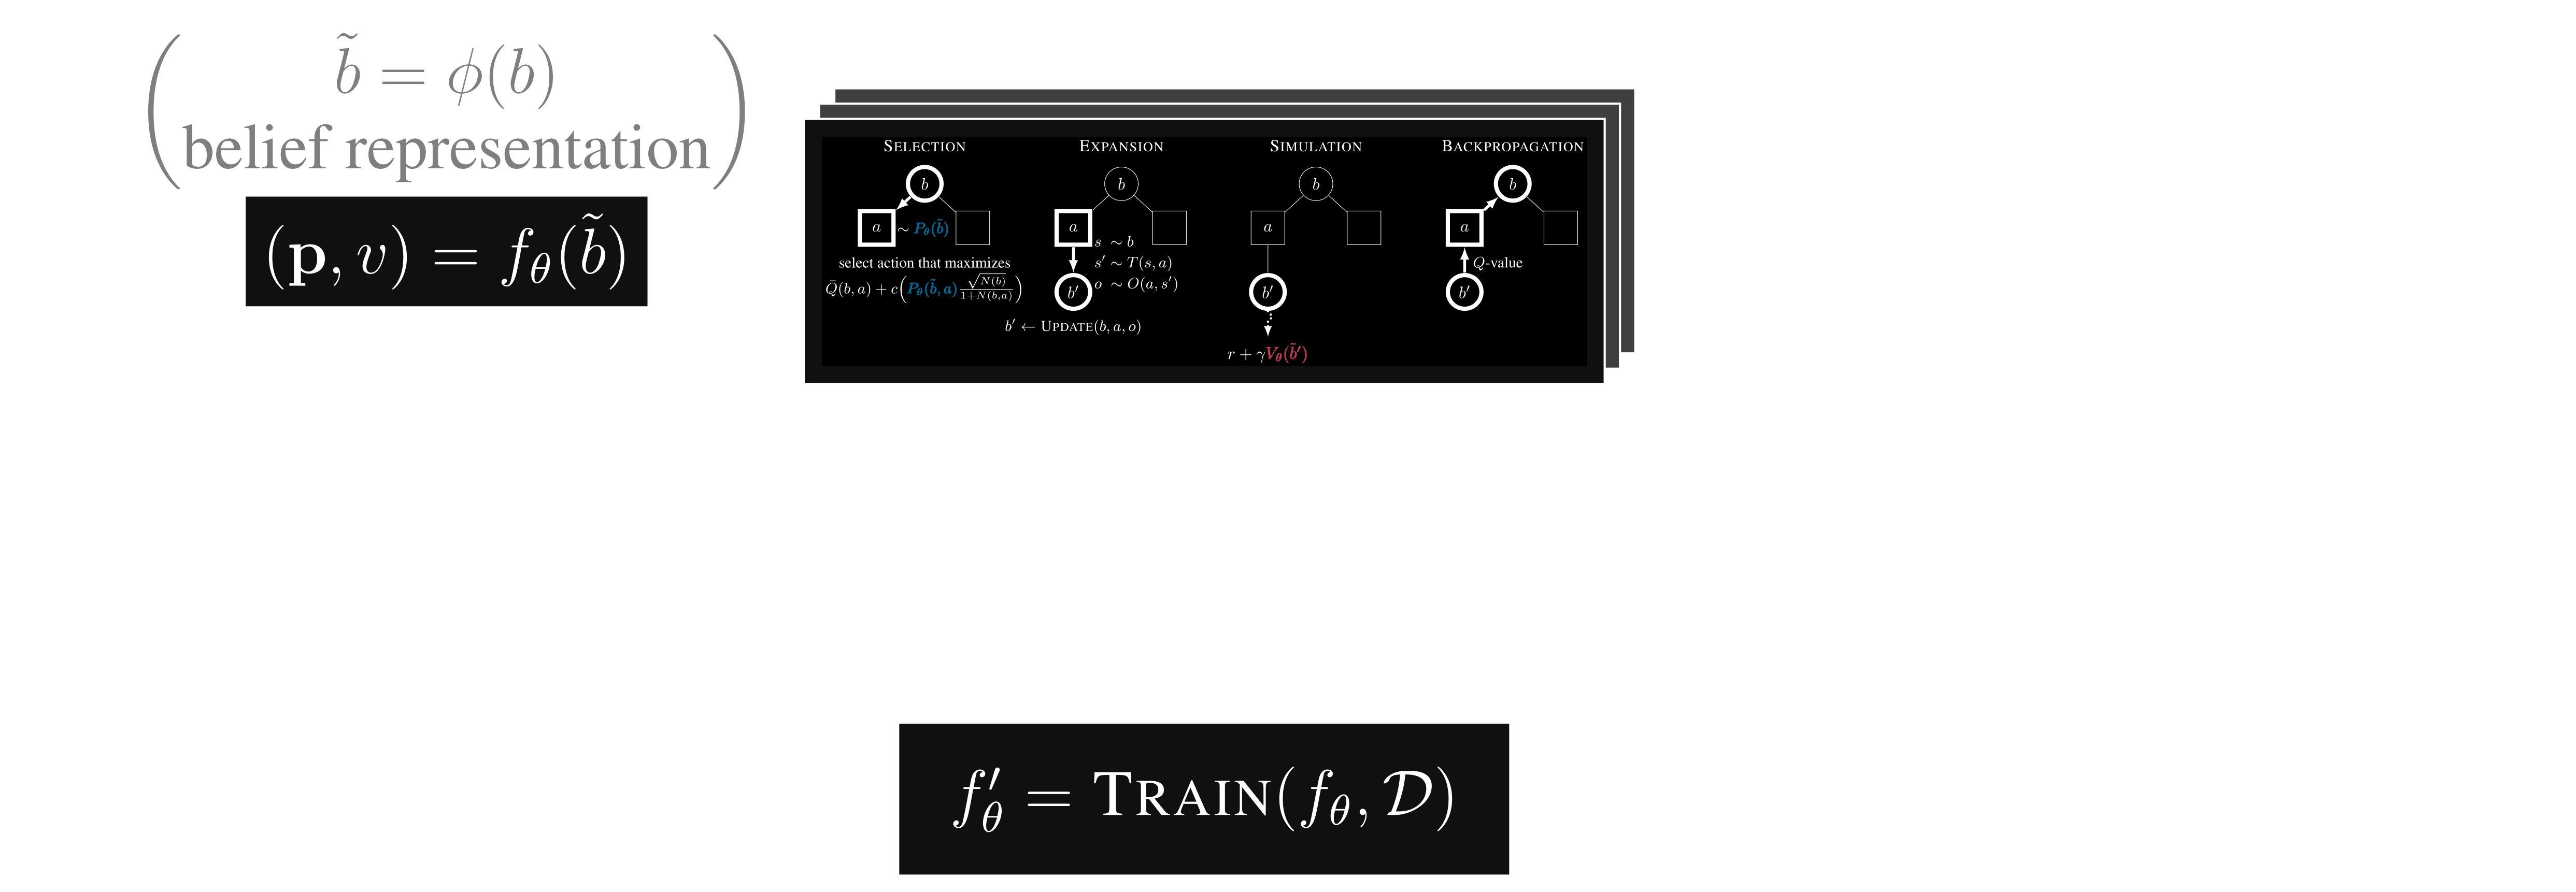
\includegraphics[height=0.4\textheight]{media/titleimage-dark.png}}
\else
    \titlegraphic{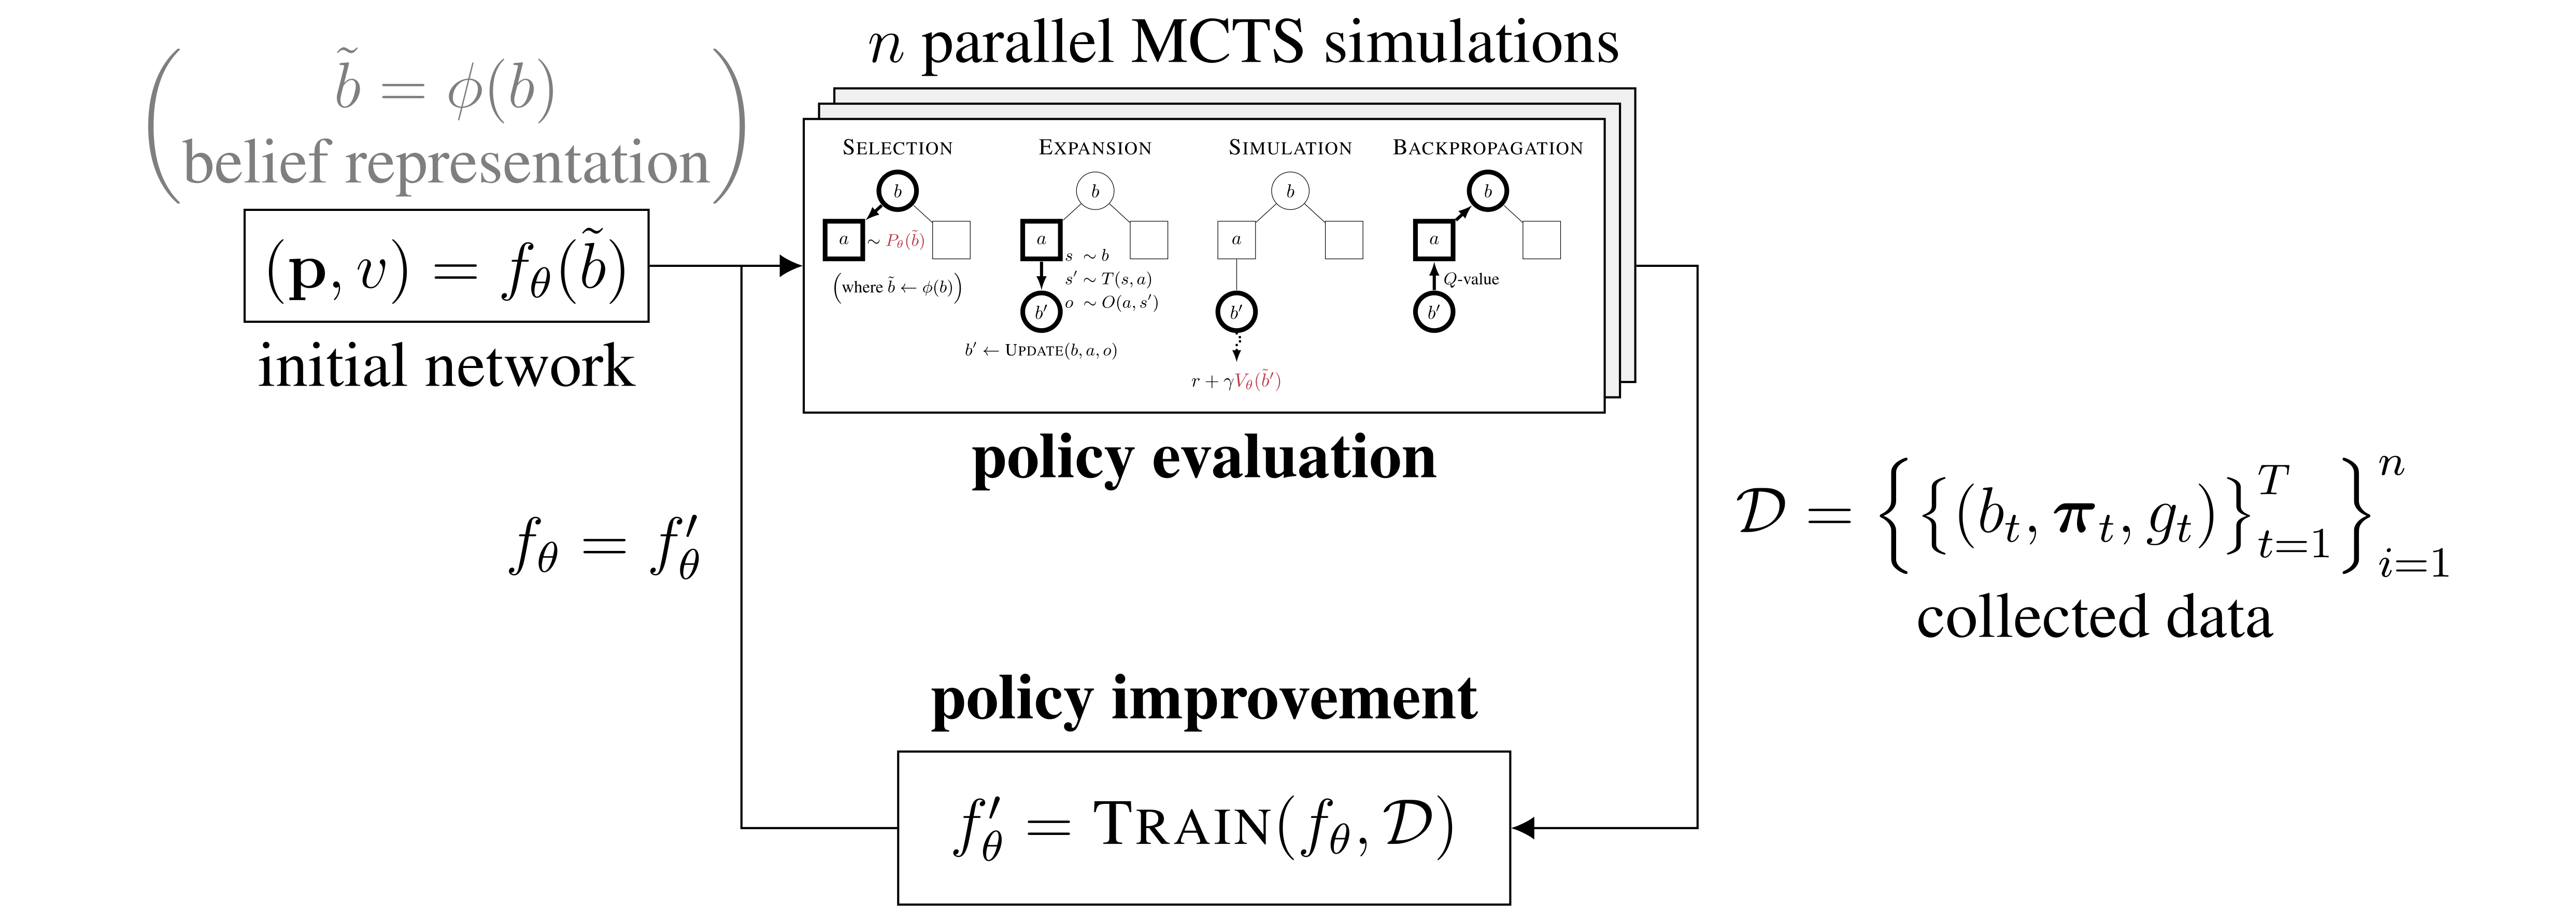
\includegraphics[height=0.4\textheight]{media/titleimage-light.png}}
\fi

\defbeamertemplate*{title page}{customized}[1][]
{
    \ifdefined\CENTERTITLE\begin{center}\fi
    \usebeamerfont{title}\textls[100]{\MakeUppercase{\textbf{\inserttitle}}}\par
    \usebeamerfont{subtitle}\usebeamercolor[fg]{subtitle}\textls[100]{\insertsubtitle}\par\par
    \ifdefined\CENTERTITLE\end{center}\fi
    \vfill
    \begin{center}
        \usebeamercolor[fg]{titlegraphic}\inserttitlegraphic
    \end{center}
    % \vfill
    \ifdefined\CENTERTITLE\begin{center}\fi
    \usebeamerfont{author}\usebeamercolor[fg]{author}\textls[100]{\insertauthor}\par
    \usebeamerfont{institute}{\usebeamercolor[fg]{institute}\textls[100]{\insertinstitute}}\par
    % \bigskip
    {\usebeamercolor[fg]{email}\@email}\par
    \usebeamerfont{date}{\usebeamercolor[fg]{date}\textls[100]{\insertdate}}\par
    \ifdefined\CENTERTITLE\end{center}\fi
}

% Small overbrace
\makeatletter
\def\smalloverbrace#1{\mathop{\vbox{\m@th\ialign{##\crcr\noalign{\kern3\p@}%
    \tiny\downbracefill\crcr\noalign{\kern3\p@\nointerlineskip}%
    $\hfil\displaystyle{#1}\hfil$\crcr}}}\limits}
\makeatother

% Small underbrace
\makeatletter
\def\smallunderbrace#1{\mathop{\vtop{\m@th\ialign{##\crcr
    $\hfil\displaystyle{#1}\hfil$\crcr
    \noalign{\kern3\p@\nointerlineskip}%
    \tiny\upbracefill\crcr\noalign{\kern3\p@}}}}\limits}
\makeatother

% Over and under arrows
\newcommand{\overarrow}[2]{\overset{\mathclap{\substack{#2 \\ \downarrow}}}{#1}}
\newcommand{\underarrow}[2]{\underset{\mathclap{\substack{\uparrow \\ #2}}}{#1}}